\title{Adversarial Examples with MNIST}
\author{
		Evan Lavender \\
		edl43@drexel.edu
}
\date{}
\documentclass[12pt]{article}
\usepackage[margin=1.0in]{geometry}
\usepackage{graphicx}
\usepackage{float}
\usepackage{amsmath}
\usepackage{cite}
\usepackage[ruled,vlined]{algorithm2e}
\usepackage{booktabs}

\begin{document}
\maketitle

\begin{abstract}
Deep neural networks have been widely implemented in a variety of tasks.
Despite this, they can be easily fooled by small intentional perturbations to their input.
These perturbations can be calculated directly using knowledge of the model, or indirectly using estimates.
The \emph{Fast Gradient Sign Method} (FGSM) and \emph{Natural Evolution Strategy} (NES) are shown to generate adversarial examples for different models.
The same techniques are used to train new models.
Including adversarial examples in the training process is shown to decrease the success rate of further adversarial attacks.

\end{abstract}

\section{Introduction}
Deep learning has made significant progress in a wide domain of tasks and is being applied in many safety-critical environments \cite{yuan2017adversarial}.
Despite this success, there are many concerns in the field of safety and security.
\cite{szegedy2013intriguing} found that they could cause a deep neural network to misclassify an image by applying a certain hardly perceptible perturbation that maximizes the network's prediction error.
They decided to call these misclassified images \emph{Adversarial Examples}.

Networks can also misclassify an image containing physical perturbations on real objects.
With a perturbation in the form of only black and white stickers, \cite{eykholt2017robust} are able to attack a real stop sign, causing targeted misclassification.
\cite{szegedy2013intriguing} suggest that this property is instrinsic to current deep neural networks.

Adversarial attacks can be categorized as either white-box or black-box.
The difference is determined by how much information the attacker is allowed to know of the network.
In a white-box attack, full knowledge of the model is allowed.
This includes architecture, inputs, outputs, weights, and gradients.
In a black-box attack, only knowledge of the inputs and outputs is allowed.

The goal of the attack can be categorized as either a misclassification or source/target misclassification.
A misclassification attack wants the output classification to be incorrect, regardless of what it actually is.
A source/target misclassification attack wants the network to predict a desired target classification.

\section{Related Work}
To generate adversarial examples, \cite{szegedy2013intriguing} used a \emph{L-BFGS} method.
This attack used an expensive linear search method which was time-consuming and impractical \cite{yuan2017adversarial}.

\cite{goodfellow2014explaining} proposed the \emph{Fast Gradient Sign Method} (FGSM).
This method is "fast" because it does not require an iterative procedure to compute examples \cite{kurakin2016adversarial}.
The sign of the gradient of the cost function with respect to the input $x$ is scaled by a hyperparameter $\epsilon$ and added to $x$ :
\begin{align*}
	& x^{adv} = x + \epsilon sign(\nabla_xJ(\hat{y}, y))
\end{align*} \cite{goodfellow2014explaining}.
The $\epsilon$ parameter controls \emph{how much} the image is allowed to change.
As the $\epsilon$ value is increased, the perturbations become more perceptible.

These are examples of white-box attack methods.
They require specific knowledge of the network in order to calculate the exact gradients needed to perturb the input.
\cite{papernot2016practical} introduce a novel black-box method in which they train a local model to substitute for the target network.
The local model is used to create adversarial examples that are misclassified by the target network \cite{papernot2016practical}.
In \cite{szegedy2013intriguing}, they found that adversarial examples genereted by one network are still statistically hard for another network, even if it was trained with different hyperparameters or on a different set of examples entirely.

\emph{Zeroth Order Optimization} (ZOO) is a different kind of black-box method by \cite{chen2017zoo}.
Instead of leveraging transferability from substitute models, ZOO-based attacks directly estimate the gradients of the targeted network.

\section{Methodology}
\subsection{Iterative Fast Gradient Sign Method}
The white-box FGSM can be extended into the \emph{Basic Iterative Method} \cite{kurakin2016adversarial}.
The "fast" method is applied multiple times with a small step size $\alpha$, with the result of each intermediate step being clipped to ensure they are in an $\epsilon$-neighborhood of the original image:
\begin{align*}
	& x_{0}^{adv} = x, x_{N+1}^{adv} = Clip_{\epsilon}\{x_{N}^{adv} + \alpha sign(\nabla_xJ(\hat{y}, y))\}
\end{align*}

\begin{algorithm}[htbp]
\SetAlgoLined
\KwIn{iterations $N$, epsilon $\epsilon$, step size $\alpha$, model $M$, input $x$, class $y$}
	$noise$ = zeros($x$.shape) \\
    \For{$i = 1, 2, 3, ... N$} {
        $x^{adv} = x + noise$ \\
		$\hat{y} = M(x^{adv})$ \\
		return $x^{adv}$ if $\hat{y} \neq y$ \\
		$noise = Clip_{\epsilon}\{noise + \alpha sign(\nabla_{x}J(\hat{y}, y))\}$
    }
\caption{Basic Iterative Method (BIM or I-FGSM)}
\label{alg:bim}
\end{algorithm}

The algorithm in \ref{alg:bim} is used for general misclassification.
If the goal is a source/target misclassification, then the algorithm can be modified in two ways.
First, $x^{adv}$ is to be returned if $\hat{y} == y$.
Second, the scaled gradient is subtracted from the $noise$.
This will cause a \emph{decrease} in the loss function for target $y$.

\subsection{Natural Evolution Strategy}
Evolution Strategies (ES) are a class of heuristic search procedures inspired by natural evolution:
At every iteration, a population of examples are perturbed and their objective function value is evaluated \cite{salimans2017evolution}.
Samples are recombined to form the population for the next iteration, until the objective is fully optimized \cite{salimans2017evolution}.

This concept can be easily applied to create adversarial examples as a black-box attack method.
The objective function being optimized is the loss function of the model, with the fitness of a sample being the value of the function.
Because an entire population of random samples is evaluated, this method is akin to estimating the gradient of the loss function using finite differences.

\begin{algorithm}[htbp]
\SetAlgoLined
\KwIn{iterations $N$, population size $n$, epsilon $\epsilon$, step size $\alpha$, sigma $\sigma$, model $M$, input $x$, class $y$}
	$\mu = 0$ \\
    \For{$i = 1, 2, 3, ... N$} {
        $noise \sim \mathcal{N}(0, I)$ \\
		$population = Clip_{\epsilon}\{\mu + \sigma * noise\}$ \\
		$fitness = $ zeros($n$) \\
		\For{$j = 0, 1, 2, ... n$} {
			$x^{adv} = x + population_j$ \\
			$\hat{y} = M(x^{adv})$ \\
			return $x^{adv}$ if $\hat{y} \neq y$ \\
			$fitness_j = J(\hat{y}, y)$ \\
		}

        $\mu = \mu + \alpha \frac{1}{n\sigma} * dot(noise.T, fitness)$ \\
    }
\caption{Natural Evolution Strategy}
\label{alg:nes}
\end{algorithm}

\subsection{Adversarial Defense}
A simple technique for building robustness against adversarial attacks is to use adversarial examples in the training data set.
During training, each sample is perturbed with a probability $p$.

\section{Evaluation}
The MNIST database \cite{lecun2010mnist} is used to evaluate both white-box (I-FGSM) and black-box (NES) attack methods.
This consists of $70000$ grayscale handwritten digits of size $28x28$.
$100$ randomly selected testing samples are used for adversarial example generation.
Each attack is allowed $500$ iterations, with epsilon values of $\epsilon = 0.1, 0.2, 0.3$, for both general misclassification and source/target misclassification.
I-FGSM uses a step size $\alpha = 0.001$, and NES uses a step size of $\alpha = 0.05$ with sigma $\sigma = 0.25$.
The median number of queries is taken using successful attacks only.

The network used is convolutional neural network based on \footnote{https://github.com/pytorch/examples/tree/master/mnist}.
Two new models are created through adversarial training and tested.
These models are created by perturbing the training data with probability $p = 0.2$ for $10$ iterations.
The attack uses a randomly generated target.
The I-FGSM and NES attacks uses a step size of $\alpha = 0.01, 0.2$ respectively.
In the table \ref{tab:my-table} below, the value on the left represents a general misclassification attack, and the value on the right is for a source/target misclassification attack.

\begin{table}[h]
\centering
\resizebox{\textwidth}{!}{%
\begin{tabular}{@{}lllllll@{}}
\toprule
 &
  \multicolumn{2}{c}{\textbf{Original}} &
  \multicolumn{2}{c}{\textbf{I-FGSM Trained}} &
  \multicolumn{2}{c}{\textbf{NES Trained}} \\ \midrule
\textbf{Test Accuracy} & \multicolumn{2}{l}{.9805} & \multicolumn{2}{l}{.9810} & \multicolumn{2}{l}{.9826} \\
                       &             &             &             &             &             &             \\
\multicolumn{7}{c}{\textbf{$\epsilon$ = 0.1}}                                                              \\
 &
  \multicolumn{1}{c}{\textbf{I-FGSM}} &
  \multicolumn{1}{c}{\textbf{NES}} &
  \multicolumn{1}{c}{\textbf{I-FGSM}} &
  \multicolumn{1}{c}{\textbf{NES}} &
  \multicolumn{1}{c}{\textbf{I-FGSM}} &
  \multicolumn{1}{c}{\textbf{NES}} \\
\textbf{Success Rate}  & 0.12/0.04   & 0.08/0.03   & 0.1/0.04    & 0.07/0.03   & 0.08/0.04   & 0.08/0.04   \\
\textbf{Query Count}   & 46/32       & 187/186     & 39/66       & 645/1321    & 40/43       & 668/867     \\
                       &             &             &             &             &             &             \\
\multicolumn{7}{c}{\textbf{$\epsilon$ = 0.2}}                                                              \\
\textbf{Success Rate}  & 0.86/0.23   & 0.43/0.08   & 0.61/0.12   & 0.38/0.03   & 0.71/0.15   & 0.40.06     \\
\textbf{Query Count}   & 171/186     & 1291/1653   & 167/189     & 1226/2133   & 161/191     & 991/2002    \\
                       &             &             &             &             &             &             \\
\multicolumn{7}{c}{\textbf{$\epsilon$ = 0.3}}                                                              \\
\textbf{Success Rate}  & 1.0/0.95    & 0.9/0.6     & 1.0/0.84    & 0.85/0.42   & 1.0/0.89    & 0.84/0.5    \\
\textbf{Query Count}   & 173/242     & 1123/1745   & 200/263     & 1251/1676   & 188/245     & 1115/1682   \\ \bottomrule
\end{tabular}%
}
\caption{Results}
\label{tab:my-table}
\end{table}

The I-FGSM outperforms the NES attack method both in terms of query count and success rate.
This is to be expected, as the white-box attack method has full knowledge of the model.
The adversarial training techniques resulted in increased testing accuracy and decreased adversarial success rate.

\begin{figure}[H]
  \centering
    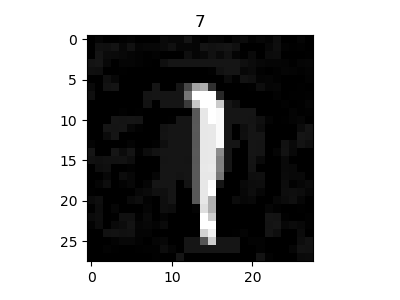
\includegraphics[width=.45\textwidth]{{../images/orig/img_50_0.10_IFGSM}.png}
    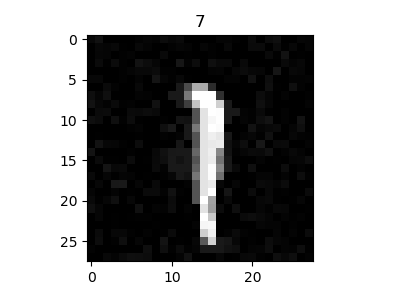
\includegraphics[width=.45\textwidth]{{../images/orig/img_50_0.10_ES}.png}
	\caption{$1 \rightarrow 7$ with $\epsilon = 0.1$}
\end{figure}

\begin{figure}[H]
  \centering
    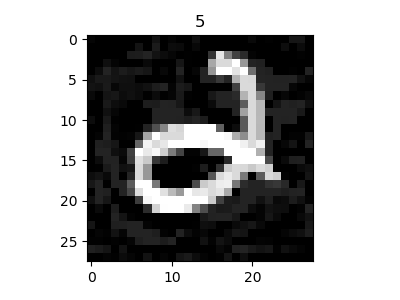
\includegraphics[width=.45\textwidth]{{../images/orig/img_29_0.20_IFGSM}.png}
    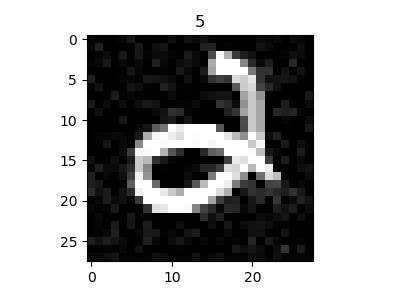
\includegraphics[width=.45\textwidth]{{../images/orig/img_29_0.20_ES}.png}
	\caption{$2 \rightarrow 5$ with $\epsilon = 0.2$}
\end{figure}

\begin{figure}[H]
  \centering
    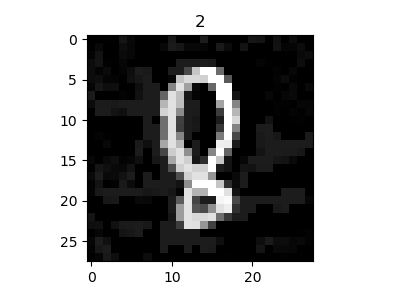
\includegraphics[width=.45\textwidth]{{../images/orig/img_8_0.30_IFGSM}.png}
    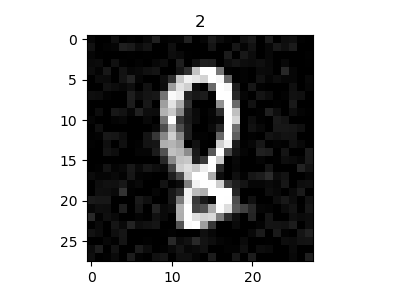
\includegraphics[width=.45\textwidth]{{../images/orig/img_8_0.30_ES}.png}
	\caption{$8 \rightarrow 2$ with $\epsilon = 0.3$}
\end{figure}

\section{Conclusions}
The \emph{Iterative Fast Gradient Sign Method} and \emph{Natural Evolution Strategy} are shown to successfully generate adversarial examples for the MNIST data set.
They are successful with the goal of general misclassification and source/target misclassification.
Using these same methods to perform adversarial training, it was shown that the resulting models were less susceptible to attack.
The test accuracy also increased as a result of the training.

\section{Future Work}
This work is just scratching the surface of the landscape of adversarial machine learning.
Aside from the task of hyperparameter tuning, there are deep questions raised by the existence of adversarial examples.
If a network can generalize well, how can it be confused by these examples, which are nearly indistinguishable from the regular examples \cite{szegedy2013intriguing}?
Questions such as this open a huge area to explore for future research.

Future paths for this work specifically include:
\begin{itemize}
	\item More data sets
	\item Experiment with using adversarial training to \emph{strengthen} actual predictions instead of lowering them.
	\item See if examples created by the original network can fool the adversarially-trained networks.
	\item Identify patterns in misclassification, i.e. what is the most likely misclassification?
\end{itemize}

\bibliographystyle{apalike}
\bibliography{refs}

\end{document}

